\chapter{绪论}

\section{引言}
\subsection{流变学的核心研究内容}
流变学是研究物质在外力作用下变形和流动的科学,其研究对象涵盖了流体、软固体以及在特定条件下可以流动的固体\cite{dealyIntroductionRheology1990}。流变学的核心在于揭示材料的应力、应变和时间之间的内在关系,并通过本构方程(流变状态方程)对这些关系进行定量描述。流变学的研究不仅深化了对材料力学行为的理解,还为工程应用和科学研究提供了重要的理论基础。流变学的核心研究内容主要包括以下几个方面\cite{elleroTanner90Years2024}:
\begin{enumerate}[topsep = 0 pt, itemsep= 0 pt, parsep=0pt, partopsep=0pt, leftmargin=44pt, itemindent=0pt, labelsep=6pt, label=(\arabic*)]
	\item 材料的流动与变形行为:材料的流动与变形行为是流变学研究的核心内容之一。通过实验和理论模型,流变学揭示了材料在外力作用下的复杂力学行为。例如,蠕变现象(即在恒定应力下,材料的变形随时间逐渐增加)和应力松弛现象(即在恒定应变下,材料的应力随时间逐渐减小)是流变学中重要的研究对象。这些现象不仅反映了材料的时间依赖性行为,还为材料的长期性能评估提供了理论依据。此外,流变学还研究了材料的非线性力学行为,如屈服、塑性变形和断裂等,这些研究对于理解材料的宏观力学性能具有重要意义。
	\item	  本构方程的构建:本构方程是流变学中用于描述材料力学行为的数学工具,其核心在于建立应力、应变和时间之间的定量关系。对于牛顿流体,其本构方程基于牛顿黏性定律,即应力与应变率成正比。然而,对于非牛顿流体和软固体,其本构方程则更为复杂,通常需要考虑材料的非线性、黏弹性以及时间依赖性等特性。通过构建合理的本构方程,流变学能够对各种物理现象进行精确的数学描述,从而为工程设计和材料开发提供理论支持。
	\item  实验与模拟方法:流变学实验是研究材料流变性能的重要手段,常见的实验方法包括蠕变实验、应力松弛实验和动力试验等。这些实验能够直接测量材料在不同条件下的力学响应,为理论模型的验证和优化提供实验数据。近年来,随着计算模拟技术的发展,流变学研究逐渐从唯象模型向定量科学转变。微观实验技术(如X射线散射、中子散射)与计算模拟的结合,使得研究者能够在微观尺度上揭示材料的流变机制,从而推动流变学向更高精度和更深层次发展。
\end{enumerate}
\subsection{流变学应用方向}
流变学的研究方向广泛,涵盖了多个学科和领域,例如高分子流变学研究高分子材料的分子结构与其流变行为的关系,例如聚合物熔体和溶液的拉伸流变行为。生物流变学研究生物材料(如血液、肌肉)的流变特性,揭示生理和病理过程中的力学机制。地质流变学研究岩石、土壤等地质材料的流变行为,应用于地震预测、矿产资源开发等领域。工业流变学在材料加工、食品工业、化妆品和医药制造等领域,流变学用于优化工艺和产品性能。非牛顿流体力学研究不符合牛顿黏性定律的流体(如油漆、泥浆、血液)的流动特性。

\section{本构方程}
\subsection{线性本构方程}
凝聚相物质分为固体或液体,固体和液体之间的一个区别特征是它们对施加的力的响应。固体在变形时储存能量,如果变形很小,则在消除力后会恢复到原来的形状。相比之下,液体则会通过耗散能量和调整其形状来抵抗力\cite{ricarteTutorialReviewLinear2024}。这种区别可以通过两种经典的力学模型来描述:胡克固体(Hookean Solid) 和牛顿流体(Newtonian Fluid)。胡克定律(Hooke's Law) 可以来描述小变形下的弹性固体行为。胡克定律表明,固体的应力$\sigma$与应变$\gamma$成正比,如公式\eqref{eq:hookean_solid}所示。其中,$G$为弹性模量,用于描述材料在弹性变形范围内抵抗外力的能力。它反映了材料的刚度,即材料在受力时发生变形的难易程度。弹性模量越大,材料越难变形;弹性模量越小,材料越容易变形。胡克固体是理想化的弹性固体模型,适用于描述金属、陶瓷等材料在小变形条件下的力学行为。
\begin{equation}
	\sigma = G \gamma  \label{eq:hookean_solid}
\end{equation}
而对于液体,其对外力的响应则完全不同。液体无法储存能量以恢复形状,而是通过内部的粘性阻力来耗散能量,并持续流动以适应外力。这种行为可以用牛顿流体的本构方程来描述,即剪切应力与剪切速率成正比,如公式\eqref{eq:newton_fluid}所示。其中,$\eta$为粘性系数,用于描述液体在运动过程中耗散能量的能力。粘性系数越大,液体越容易耗散能量,反之亦然。牛顿流体是理想化的粘性流体模型,适用于描述水、空气等液体在运动过程中耗散能量的行为。
\begin{equation}
	\sigma = \eta \dot{\gamma}  \label{eq:newton_fluid}
\end{equation}
然而,这些特征都是理想化的,代表了特定条件的行为。许多凝聚相材料不容易归入这些经典类别,因为它们的机械性能取决于变形的大小、速率、变形历史,加载过程等等。例如,考虑牙膏,它像液体一样流动,可以将其从管中挤出,但一旦放在牙刷上,它就会像固体一样保持其形状。这类物质同时具有黏性和弹性,被认为是黏弹性材料,被称为软物质或者复杂流体。

线性黏弹性理论认为在小变形范围(线性范围内)应力-应变关系是线性的,即应力与应变成正比。同时线性黏弹性区间内材料具有时间依赖性,材料的力学响应不仅取决于当前的应力或应变,还依赖于时间或加载历史。
\begin{figure}[htbp]
	\centering
	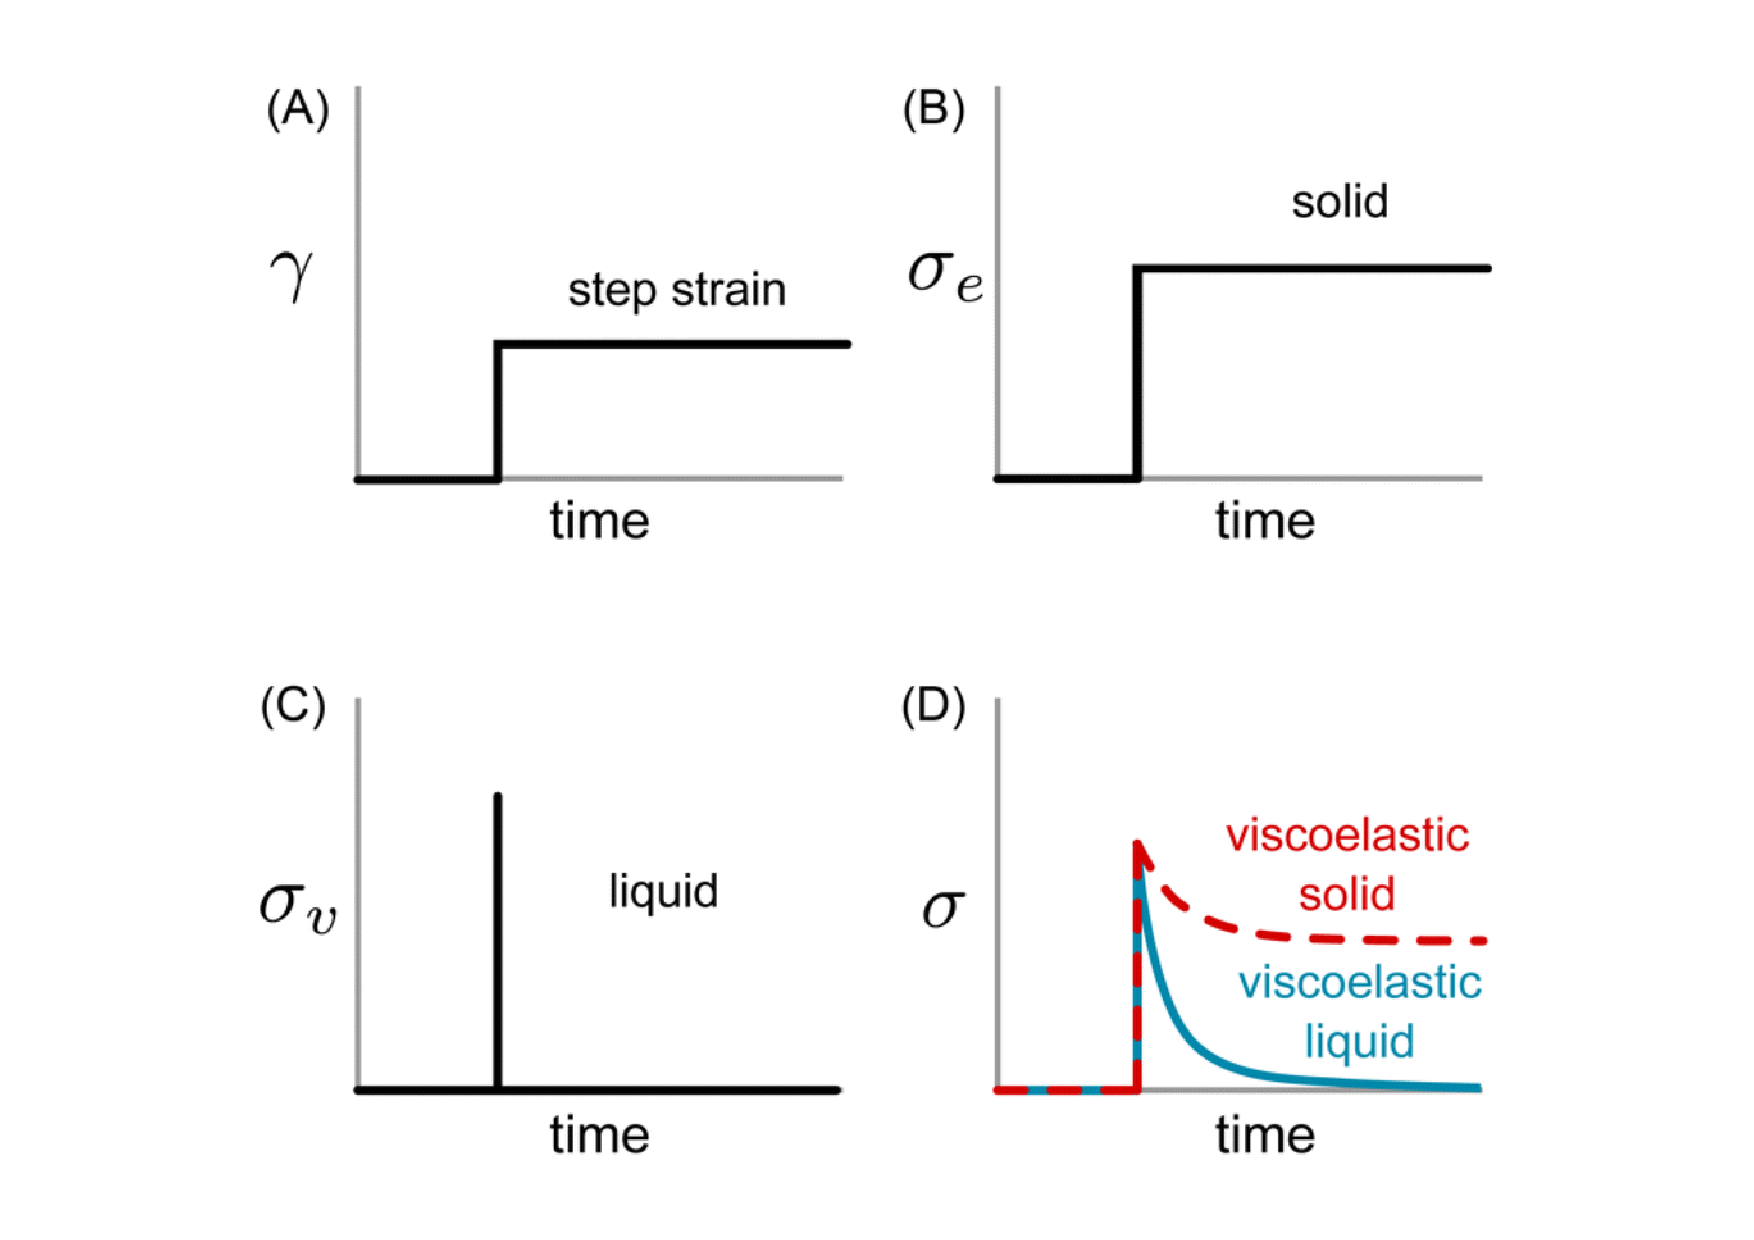
\includegraphics[width=\textwidth]{Fig/solid_liquid.pdf}
	\FigureBicaption{\label{differ_fluid_intro}(A)施加的应变曲线以及对应的剪切应力;(B)理想弹性固体;(C)理想粘性液体;(D)粘弹性样品\cite{ricarteTutorialReviewLinear2024}}{(A) Applied strain profile and resulting shear stress;(B) ideal elastic solid;(C) ideal viscous liquid;(D) viscoelastic samples\cite{ricarteTutorialReviewLinear2024}}
\end{figure}
图\ref{differ_fluid_intro}概述了两种不同类型的粘弹性材料的简单剪切行为。对于粘弹性固体和液体,阶跃应变会引起瞬时弹性响应,从而产生σ峰值。然而,应力不是保持不变或立即降至零,而是逐渐降低。它在很长一段时间内接近粘弹性固体的有限平台值,而粘弹性液体则完全衰减到零\cite{ricarteTutorialReviewLinear2024}。

线性本构理论中最经典的是Maxwell模型,如图\ref{maxwell_intro}所示,Maxwell模型将材料的弹性行为和粘性行为结合起来,它用一个弹簧(弹性元件)和一个粘壶(粘性元件)串联表示黏弹性关系。Maxwell模型的微分形式如公式\eqref{eq:maxwell_model_dt}所示,其中$\tau$表示松弛时间,等于$eta/G$。将两边积分得到Maxwell模型的积分形式如公式\eqref{eq:maxwell_model_int}所示。
\begin{align}
	 & \frac{d\sigma}{dt} + \frac{\sigma}{\tau}  = G \frac{d\gamma}{dt} \label{eq:maxwell_model_dt}                                                   \\
	 & \sigma(t)                                = \int_{-\infty}^{t} G e^{-\frac{t-t'}{\tau}} \frac{d\gamma(t')}{dt'} dt'\label{eq:maxwell_model_int}
\end{align}
积分形式的方程显示了任何时刻的应力是松弛模量乘以应变速率的积分,该时刻之前材料的整个历史。由于被积函数中的衰减指数,模型具有衰落的记忆,因此最近的应变历史比过去的应变历史更重要。
\begin{figure}[htbp]
	\centering
	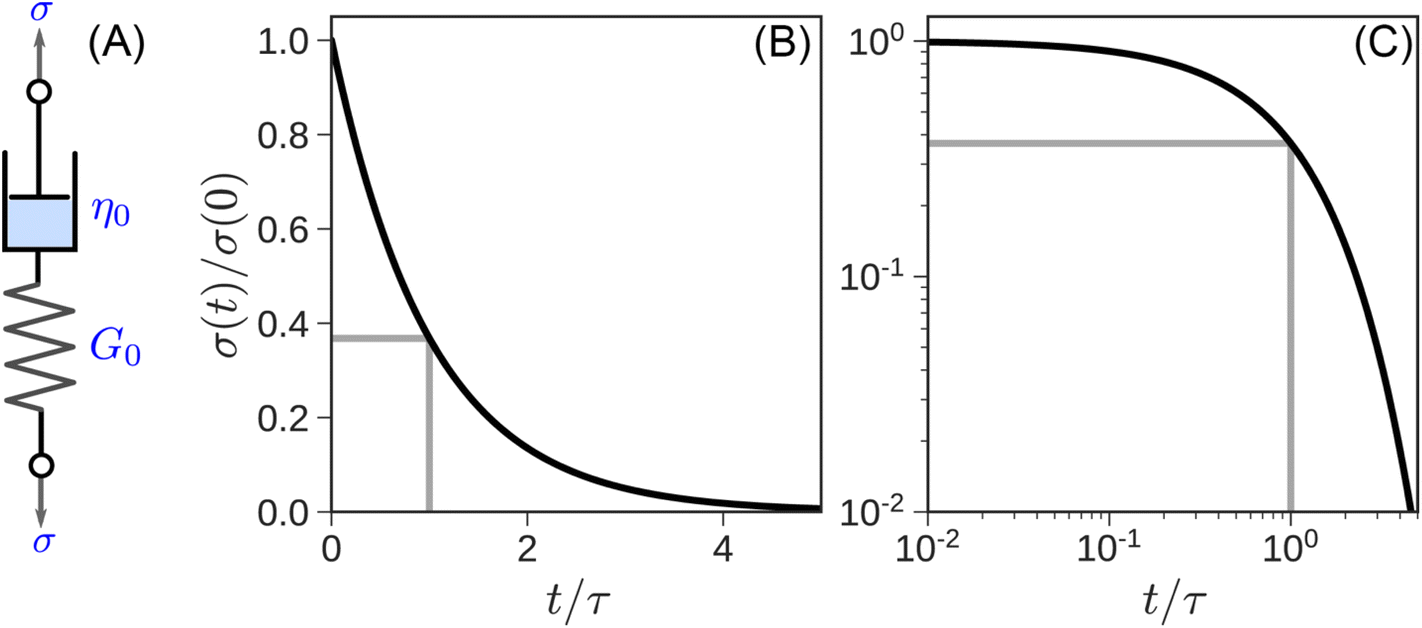
\includegraphics[width=0.8\textwidth]{Fig/maxwell_intro.png}
	\FigureBicaption{\label{maxwell_intro} Maxwell 模型示意图}{Maxwell model schematic}
\end{figure}
如果将多个Maxwell模型并联,便可以得到广义Maxwell模型方程,如公式\eqref{eq:generalized_maxwell_model}所示。
\begin{equation}
	\sigma(t) = \int_{-\infty}^{t} G(t-t') \frac{d\gamma(t')}{dt'} dt' \label{eq:generalized_maxwell_model}
\end{equation}
其中松弛模量 \(G(t)\) 定义为公式\eqref{eq:generalized_maxwell_model_G}。
\begin{equation}
	G(t) = \sum_{i=1}^{n} G_i e^{-\frac{t}{\tau_i}} \label{eq:generalized_maxwell_model_G}
\end{equation}

Maxwell模型通过将黏弹性抽象为黏性元件和弹性元件串联来得到本构方程。如果将弹簧和粘壶进行并联,则得到Kelvin-Voigt 模型的本构方程,即公式\eqref{eq:kelvin_voigt_model}。
\begin{equation}
	\sigma(t) = G \gamma(t) + \eta \frac{d\gamma(t)}{dt} \label{eq:kelvin_voigt_model}
\end{equation}
将多个Kelvin-Voigt模型的元件进行串联,便可以得到广义Kelvin-Voigt模型,如公式\eqref{eq:generalized_kelvin_voigt_model}。
\begin{equation}
	\sigma(t) = \sum_{i=1}^{n} \left( G_i \gamma_i(t) + \eta_i \frac{d\gamma_i(t)}{dt} \right)\label{eq:generalized_kelvin_voigt_model}
\end{equation}
原则上,任何广义Voigt模型都可以在数值上映射到等效的广义 Maxwell模型,这是线性本构方程构建的基本研究方法的不同角度。

如果将传统的整数阶导数模型改为分数阶导数,能够更加准确描述材料的记忆效应,即材料的当前状态不仅依赖于当前时刻的输入,还依赖于过去的历史。这种特性在黏弹性材料中非常重要,因为材料的应力或应变响应通常具有时间依赖性。例如Bagley和Torvik等在20世纪80年代提出的分数阶Maxwell模型,是对传统Maxwell模型的推广。无论是什么形式的线性本构方程,均满足一个基本假设材料的响应是线性的,即多个应变历史的叠加效应等于各自效应的线性相加,当公式\eqref{eq:generalized_maxwell_model}中的松弛模量G表示为公式\eqref{eq:generalized_maxwell_model_G}时是Maxwell模型的形式,事实上当G为一个抽象的松弛函数时,公式\eqref{eq:generalized_maxwell_model}抽象为更一般的线性本构方程,被称为玻尔兹曼叠加原理(BSP),玻尔兹曼叠加原理广泛应用于描述线性黏弹性材料的行为,例如应力松弛、蠕变、动态力学响应等。
\subsection{非线性本构方程}
线性本构方程只能用于描述只能描述简单的材料行为,例如弹性变形、小应变下的黏弹性行为。适用于材料在小变形范围内的线性响应。能够描述复杂的材料行为,而非线性本构方程可以用来描述更为复杂的行为例如塑性变形、硬化或软化、各向异性、大变形、剪切稀化、剪切增稠等行为。绝大部分高分子材料具有较复杂的非线性关系。Binham提出模型认为屈服性流体当剪应力低于屈服应力时,流体表现为刚性固体;当剪应力超过屈服应力时,流体开始流动,且流动行为类似于牛顿流体.Herschel-Bulkley模型在此基础之上引入了剪切稀化和剪切增稠的表示,如公式\eqref{eq:herschel},是描述非线性本构方程的一套公式。
\begin{equation}
	\sigma=\sigma_0+K\dot{\gamma}^n \label{eq:herschel}
\end{equation}
松弛模量函数不仅是时间的函数,也是应变的函数,能够表征大变形下的非线性响应。改进的Bingham模型在Herschel-Bulkley模型的基础上,通过引入额外的参数或修正项,显著提升了对流体行为的描述精度。例如,在Herschel-Bulkley模型中引入高阶项(如剪切速率的二阶项),可以更准确地刻画非线性流变行为。此外,通过引入Papanastasiou正则化方法,有效解决了原始模型在低剪切速率下的数值不稳定性问题,这一改进模型被称为Herschel-Bulkley-Papanastasiou (HBP) 模型。HBP模型在磁流变液等复杂流体的流变特性描述中得到了广泛应用。
Herschel-Bulkley类模型不涉及弹性流体,主要用于解决屈服应力流体的本构问题,对于黏弹性流体的非线性本构方程而言,可以写出一般的通式,如公式\eqref{eq:nolinear_model},非线性黏弹性流体的本构方程可以从宏观连续介质力学和微观分子角度分别进行描述。
\begin{equation}
	\sigma(t) = \int_{-\infty}^{t} G(t-t',\gamma) \frac{d\gamma(t')}{dt'} dt' \label{eq:nolinear_model}
\end{equation}

宏观介质力学中Oldroyd-B模型,如公式\eqref{eq:oldroyd_b}是在Maxwell模型的基础上作了修正,增加了延迟时间项$\lambda_2$ ,从而能够描述更复杂的流变行为,同时这个模型引入了上随体导数来代替普通导数,在物理上更加符合真实世界的材料行为。Oldroyd-B模型本意可以在Weissenberg数($W_i=\lambda_1 \dot{\gamma}_i$)较小的情况下描述线性黏弹性,但是其中的上随体导数在一定程度上包含了部分非线性效应,特别是在高应变率或大变形条件下。Oldroyd-B模型是非线性本构方程的经典基础模型,研究者在此基础上为了更准确地描述非线性黏弹性行为,研究者提出了多种修正的 Oldroyd-B模型。
\begin{equation}
	\boldsymbol{\sigma} + \lambda_1 \frac{\mathcal{D}\boldsymbol{\sigma}}{\mathcal{D}t} = \eta \left( \dot{\boldsymbol{\gamma}} + \lambda_2 \frac{\mathcal{D}\dot{\boldsymbol{\gamma}}}{\mathcal{D}t} \right) \label{eq:oldroyd_b}
\end{equation}
Giesekus模型(公式\eqref{eq:giesekus})在Oldryd-B模型基础上,增加了一个非线性项,通过非线性系数$\alpha$来表示非线性行为。Giesekus模型常用于描述高聚物溶液、熔体以及其他粘弹性流体的流变行为。这些流体通常表现出剪切稀化和弹性效应。尤其是在中等至高剪切速率范围内。其模型参数(如迁移因子α)可以调节剪切稀化的强度和拐点形状,具有较高的灵活性。Giesekus模型在高Weissenberg数(Wi)条件下仍能保持数值稳定性,适用于强弹性效应的流动场景。通过引入对数构象重构等方法,可以进一步提高其在高Wi条件下的计算稳定性。
\begin{equation}
	\boldsymbol{\sigma} + \lambda_1 \frac{\mathcal{D}\boldsymbol{\sigma}}{\mathcal{D}t} + \alpha \frac{\lambda_1}{\eta} \boldsymbol{\sigma} \cdot \boldsymbol{\sigma} = \eta \left( \dot{\boldsymbol{\gamma}} + \lambda_2 \frac{\mathcal{D}\dot{\boldsymbol{\gamma}}}{\mathcal{D}t} \right) \label{eq:giesekus}
\end{equation}
PTT模型(公式\eqref{eq:ptt})通过引入一个非线性应力函数$f$扩展了Oldroyd-B模型。该函数通常取指数形式。
\begin{equation}
	f(\text{tr}(\boldsymbol{\sigma})) \boldsymbol{\sigma} + \lambda_1 \frac{\mathcal{D}\boldsymbol{\sigma}}{\mathcal{D}t} = \eta \left( \dot{\boldsymbol{\gamma}} + \lambda_2 \frac{\mathcal{D}\dot{\boldsymbol{\gamma}}}{\mathcal{D}t} \right) \label{eq:ptt}
\end{equation}
FENE-P模型(公式\eqref{eq:fene_p})在 Oldroyd-B 模型的基础上引入了有限拉伸效应,通过项$\frac{\lambda_1}{\eta} \frac{\boldsymbol{\sigma}}{1 - \text{tr}(\boldsymbol{\sigma})/b}$描述聚合物链的有限拉伸行为。参数$b$表示聚合物链的最大拉伸比。该模型适用于描述聚合物溶液在强流动条件下的非线性行为。
\begin{equation}
	\boldsymbol{\sigma} + \lambda_1 \frac{\mathcal{D}\boldsymbol{\sigma}}{\mathcal{D}t} = \eta \left( \dot{\boldsymbol{\gamma}} + \lambda_2 \frac{\mathcal{D}\dot{\boldsymbol{\gamma}}}{\mathcal{D}t} \right) - \frac{\lambda_1}{\eta} \frac{\boldsymbol{\sigma}}{1 - \text{tr}(\boldsymbol{\sigma})/b} \label{eq:fene_p}
\end{equation}
通过将Oldroyd-B模型与分数阶导数结合,可以得到分数阶Oldroyd-B模型,如公式\eqref{eq:fractional_oldroyd_b}。分数阶 Oldroyd-B模型通过引入分数阶导数描述非局部记忆效应。参数$\alpha$和$\beta$是分数阶导数的阶数,该模型能够捕捉更复杂的流变行为,适用于具有非局部记忆效应的复杂流体。
\begin{equation}
	\boldsymbol{\sigma} + \lambda_1^\alpha \frac{\mathcal{D}^\alpha \boldsymbol{\sigma}}{\mathcal{D}t^\alpha} = \eta \left( \dot{\boldsymbol{\gamma}} + \lambda_2^\beta \frac{\mathcal{D}^\beta \dot{\boldsymbol{\gamma}}}{\mathcal{D}t^\beta} \right) \label{eq:fractional_oldroyd_b}
\end{equation}
Oldroyd-B类本构模型均为微分型本构模型,源于微分型Maxwell模型公式\eqref{eq:maxwell_model_dt}。另一类本构模型如K-BKZ模型源于积分型Maxwell模型公式\eqref{eq:maxwell_model_int}。
K-BKZ模型如公式\eqref{eq:k_bkz_model}所示。在 K-BKZ 模型中,$h$ 称为阻尼函数,它是形变张量的第一不变量 $I_1$ 和第二不变量 $I_2$ 的函数。$\mathbf{C}^{-1}(t,t')$ 是Finger 形变张量的逆,用于描述从时间 $t'$ 到 $t$ 的形变历史。$m(t-t')$ 是瞬态函数或记忆函数,用于表征材料对历史形变的记忆效应。K-BKZ 模型广泛应用于聚合物加工(如挤出、注塑、热成型等)、生物流体力学(如血液、蛋白质悬浮液等复杂流体的流变行为研究)以及涂料和润滑剂的流动行为和流变特性分析。
\begin{align}
	% K-BKZ 模型基本形式
	 & \boldsymbol{\sigma}(t)  = \int_{-\infty}^t m(t-t') \, h(I_1, I_2) \, \mathbf{C}^{-1}(t,t') \, dt'    \label{eq:k_bkz_model}
\end{align}

Doi和Edwards尝试从分子角度构建本构方程,在管子模型的基础上提出了Doi-Edwards模型(公式\eqref{eq:doi_edwards})。Doi-Edwards 模型的核心思想是将高分子链的缠结效应简化为一条光滑管道对链的限制作用,链在管道中的运动通过松弛和扩散来描述。其中$G_0$表示松弛时间,而$Q$表示为公式\eqref{eq:doi_edwards_q},反映了高分子链在形变历史下的方向分布变化,即链的取向如何随形变而变化。
\begin{align}
	 & \boldsymbol{\sigma}(t)  = G_0 \int_{-\infty}^t \frac{\partial Q(\mathbf{E}(t,t'))}{\partial t'} \, dt'    \label{eq:doi_edwards}                                                                  \\
	 & Q(\mathbf{E}(t,t'))     = \frac{5}{2} \left\langle \frac{\mathbf{E}(t,t') \cdot \mathbf{u} \mathbf{u}}{|\mathbf{E}(t,t') \cdot \mathbf{u}|^2} \right\rangle_{\mathbf{u}} \label{eq:doi_edwards_q}
\end{align}
传统的 Doi-Edwards模型基于单链平均场近似,将缠结效应简化为一条光滑的“管子”对高分子链的限制作用。然而,这种简化忽略了链-链间的直接相互作用,难以解释快速大形变条件下的非线性流变现象(如应力过冲、缠结点破损和重组等)。近年来,研究者通过引入多链相互作用,提出了修正的管子模型,例如 GLaMM 理论,在此基础之上能够更好地描述缠结高分子流体的非线性行为。

\subsection{传统的本构方程的构建方法}
传统本构方程尤其是Oldroyd-B、Doi-Edwards等复杂的非线性模型具有较多的待定参数,通过数学形式描述材料的应力-应变关系及其对时间、温度和形变历史的依赖性。其构建方法主要基于实验观测、理论推导和数值模拟的结合,通常分为以下几个步骤。

首先,实验观测是构建本构方程的基础。通过流变学实验(如剪切流变、拉伸流变等),研究者可以获取材料在不同形变条件下的应力响应数据。这些实验数据为理论模型的构建提供了关键依据。例如,通过动态力学分析(DMA)测量材料的存储模量和损耗模量,可以确定其粘弹性特性;通过应力松弛和蠕变实验,可以推断材料的记忆效应和时间依赖性。实验数据的精确性和全面性直接决定了本构方程的适用性和预测能力。

其次,理论推导是本构方程构建的核心环节。对于线性粘弹性材料,通常采用弹簧和粘壶的组合模型(如 Maxwell 模型、Kelvin-Voigt 模型)来描述其力学行为,通过不同的组合可以表示不同的本构方程。对于非线性材料,则需要引入更复杂的本构关系,这里主要还是基于线性黏弹性方程,通过各类引入非线性关系的方法来进行非线性关系推导,理论推导的关键在于如何将微观结构信息(如高分子链的缠结、颗粒的相互作用等)与宏观力学行为联系起来。而对于理论推导的结果,每一个非线性项或参数应当从数学角度进行证明。例如近年来,数学研究者对Doi-Edwards模型的适定性进行了深入研究。Chupin等人通过Schauder不动点定理和Galerkin近似方法,证明Doi-Edwards 模型在二维情况下的全局解存在性和唯一性。这一结果为模型的数学基础提供了严格的理论支持。

此外,数值模拟在本构方程的构建和验证中起到了重要作用。有限元分析(FEA),有限有限差分法 (FDM) ,有限体积法(FVM)是一种常用的数值方法,能够将本构方程嵌入到复杂几何和边界条件下的力学问题中,模拟材料的应力分布、形变行为和流动特性。例如,在聚合物加工中,研究者通过有限元分析结合 Doi-Edwards 模型,可以预测熔体在挤出或注塑过程中的流动行为,优化加工参数。分子动力学模拟(MD)则是另一种重要的数值工具,能够从分子尺度模拟材料的力学行为,为宏观本构方程的构建提供微观依据。例如,通过粗粒度分子动力学模拟(CGMD),研究者可以研究高分子链的缠结动力学,验证管子模型的假设。由于聚合物液体具有单体、中观和宏观流尺度的多尺度特征,因此关联不同层次的多尺度模拟(MSS)足以准确再现流动特性
\begin{figure}[htbp]
	\centering
	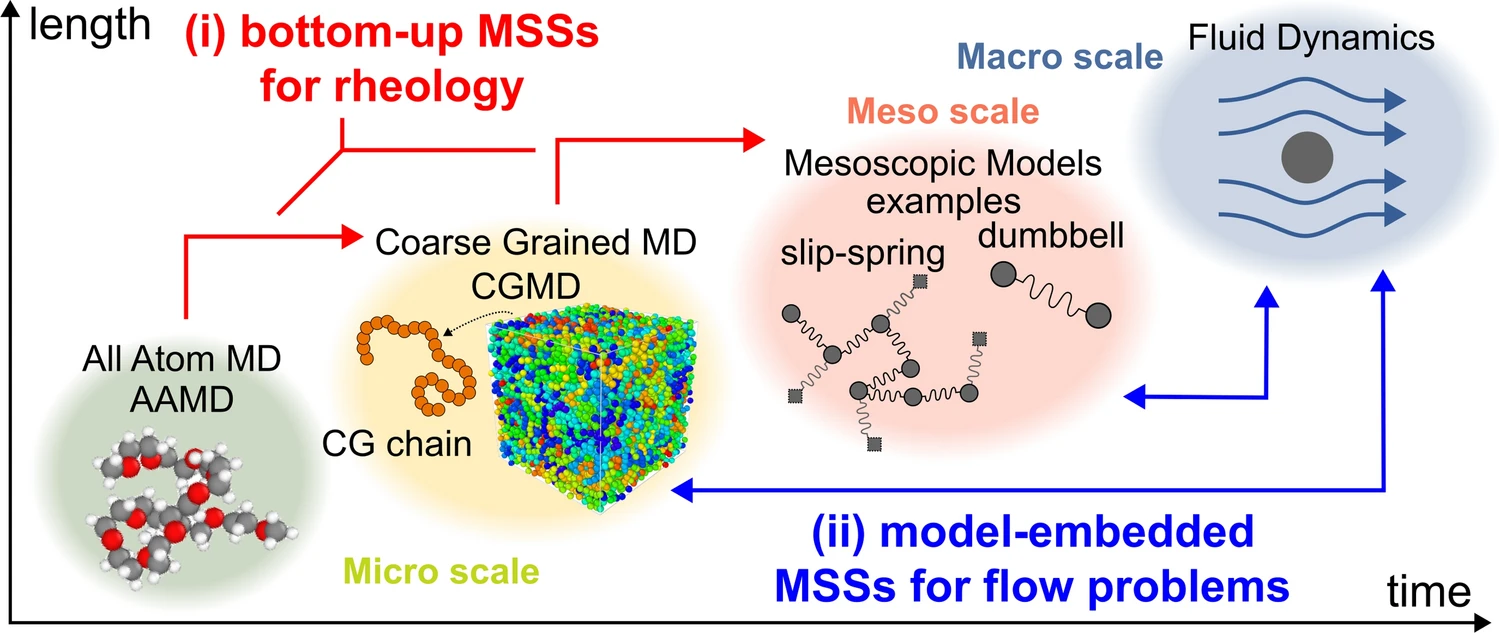
\includegraphics[width=0.8\textwidth]{Fig/duochidumoni.png}
	\FigureBicaption{\label{duochidumoni} 多尺度模拟}{MSS}
\end{figure}

传统本构方程的研究方法主要依赖于物理实验和理论推导,通过建立数学方程来描述材料的力学行为。这种方法虽然具有明确的物理意义,但在处理复杂材料或非线性行为时,往往面临模型精度不足、参数识别困难等问题。随着数据驱动技术的快速发展,机器学习为材料本构关系的研究提供了新的思路。通过利用大量实验或仿真数据,机器学习能够自动挖掘材料行为中的潜在规律,构建高精度的预测模型,从而弥补传统方法的不足,并为材料科学的研究开辟了更加智能化的路径。
\section{机器应用于本构方程研究现状}
\subsection{机器学习方法介绍}
机器学习是人工智能的一个重要分支,其核心是通过算法从数据中自动学习规律,并利用这些规律进行预测或决策。与传统编程不同,机器学习不依赖于明确的规则,而是通过训练数据优化模型参数,从而实现对复杂问题的建模和解决。它在图像识别、自然语言处理、推荐系统等领域取得了显著成果。

监督学习是最常见的机器学习类型,适用于有标签的数据集。常见的算法包括线性回归和逻辑回归,分别用于连续值的预测和二分类问题。决策树通过树状结构进行决策,适用于分类和回归任务。随机森林是多个决策树的集成,通过投票或平均提高预测准确性。支持向量机(SVM)通过寻找最优超平面进行分类,适用于高维数据。K近邻算法(KNN)基于距离度量进行分类或回归,简单但计算量大。朴素贝叶斯基于贝叶斯定理,适用于文本分类等任务。无监督学习则更多处理无标签数据,主要用于数据聚类和降维。

随着数据规模和计算能力的提升,深度学习作为机器学习的一个子领域迅速崛起。深度学习通过构建多层的神经网络结构,能够自动提取数据中的多层次特征,从而在处理高维、非线性问题(如图像、语音和文本)时表现出更强的能力,成为推动人工智能发展的核心技术之一。
卷积神经网络(CNN)通过卷积层提取图像特征,广泛应用于图像分类和目标检测。循环神经网络(RNN)及其变体LSTM和GRU,适用于序列数据如时间序列和自然语言处理。Transformer模型通过自注意力机制处理长序列,成为自然语言处理的主流架构。生成对抗网络(GAN)通过生成器和判别器的对抗训练,能够生成逼真的图像和文本。
\subsection{数据驱动方法}
近年来在物理学领域,机器学习与物理学问题的研究结合也日益密切。在流变学领域,人工神经网络(ANN)已被用于自动监测合成油基泥浆的各种流变特性。混合ML模型结合了ANN和支持向量机(SVM)准确预测了纳米基水基钻井液的流变性和过滤特性。此外,ML模型可以与微流体或其他设备集成,用于复杂流体的原位粘度测量。例如,Mustafa等设计了一种微流体传感设备,利用流固耦合和 ML 算法来测量复杂流体的粘度。他们采用SVM和 (KNN)算法,分别实现了 89.7\%和 98.9\% 的平均准确率。Ponick 等利用卷积神经网络(CNN)通过立体相机图像预测 Bingham 流体的流变特性。
\subsection{引入物理约束的神经网络研究}
物理约束神经网络研究通过引入物理约束,将本构方程嵌入到复杂几何和边界条件下的力学问题中,模拟材料的应力分布、形变行为和流动特性。例如,在聚合物加工中,研究者通过有限元分析结合 Doi-Edwards 模型,可以预测熔体在挤出或注塑过程中的流动行为,优化加工参数。分子动力学模拟(MD)则是另一种重要的数值工具,能够从分子尺度模拟材料的力学行为,为宏观本构方程的构建提供微观依据。例如,通过粗粒度分子动力学模拟(CG)
\section{本课题研究介绍}
\subsection{研究内容}
本课题研究通过利用机器学习算法,对多尺度材料本构方程进行深度学习研究,以解决多尺度材料本构方程的数值问题。通过引入物理约束,将本构方程嵌入到复杂几何和边界条件下的力学问题中,模拟材料的应力分布、形变行为和流动特性。例如,在聚合物加工中,研究者通过有限元分析结合 Doi-Edwards 模型,可以预测熔体在挤出或注塑过程中的流动行为,优化加工参数。分子动力学模拟(MD)则是另一种重要的数值工具,能够从分子
\subsection{创新之处}
本课题研究通过利用机器学习算法,对多尺度材料本构方程进行深度学习研究,以解决多尺度材料本构方程的数值问题。通过引入物理约束,将本构方程嵌入到复杂几何和边界条件下的力学问题中,模拟材料的应力分布、形变行为和流动特性。例如,在聚合物加工中,研究者通过有限元分析结合 Doi-Edwards 模型,可以预测熔体在挤出或注塑过程中的流动行为,优化加工参数。分子动力学模拟(MD)则是另一种重要的数值工具,能够从分子
\subsection{研究意义}
研究意义是解决多尺度材料本构方程的数值问题,提高材料科学研究效率,为材料工程师提供更好的工具。


